\documentclass[a4paper, 11pt]{article}
\usepackage{comment} % enables the use of multi-line comments (\ifx \fi) 
\usepackage{xparse}% http://ctan.org/pkg/xparse
\NewDocumentCommand{\Log}{o}{%
  \IfNoValueTF{#1}{}{{}^{#1}\!}\log}%
  
\usepackage{fullpage} % changes the margin
\usepackage{longtable}
\usepackage{graphicx}
\usepackage{fancyvrb,xcolor}
\usepackage{listings}
\usepackage{color}
\usepackage[hyphenbreaks]{breakurl}
\usepackage[hyphens]{url}
\usepackage[margin=3cm]{geometry}
\usepackage{relsize}
\definecolor{dkgreen}{rgb}{0,0.6,0}
\definecolor{gray}{rgb}{0.5,0.5,0.5}
\definecolor{mauve}{rgb}{0.58,0,0.82}
\usepackage{float}
\usepackage{caption}
\DeclareCaptionFont{white}{\color{white}}
\DeclareCaptionFormat{listing}{\colorbox{gray}{\parbox{\textwidth}{#1#2#3}}}
\captionsetup[lstlisting]{format=listing,labelfont=white,textfont=white}
\newcommand{\bigqm}[1][1]{\text{\larger[#1]{\textbf{?}}}}
\lstset{
  language=Java,
  aboveskip=3mm,
  belowskip=3mm,
  showstringspaces=false,
  columns=flexible,
  basicstyle={\small\ttfamily},
  numbers=none,
  numberstyle=\tiny\color{gray},
  keywordstyle=\color{blue},
  commentstyle=\color{dkgreen},
  stringstyle=\color{mauve},
  breaklines=true,
  breakatwhitespace=true,
  tabsize=3
}
\graphicspath{ {images/} }

\begin{document}
%Header-Make sure you update this information!!!!
\noindent
\large\textbf{Assignment 5} \hfill \textbf{Hussam Hallak} \\
\normalsize CS532, Web Science, Spring 2017\hfill CS Master's Student \\
Old Dominion University, Computer Science Dept \hfill Prof: Dr. Nelson 

\section*{Question 1:}
We know the result of the Karate Club (Zachary, 1977) split.
Prove or disprove that the result of split could have been predicted
by the weighted graph of social interactions.  How well does the
mathematical model represent reality?

Generously document your answer with all supporting equations, code,
graphs, arguments, etc.

\subsection*{Answer:}
I started by plotting the Karate Club social interaction graph prior to the fission. I wrote a simple R script to plot the graph.

\begin{lstlisting}[language=R, breakatwhitespace=〈false), label=Karate Club Social Interaction Graph Before Club Fission in R, caption= Karate Club Social Interaction Graph Before Club Fission in R]
> library(igraph)
> library(igraphdata)
> data(karate)
> plot.igraph(karate, 
+             vertex.color="yellow",
+             vertex.size = 10,
+             main="Karate Club Social Interaction Graph Before Club Fission"
+ )
>
\end{lstlisting}

\begin{figure}[H]
\centering
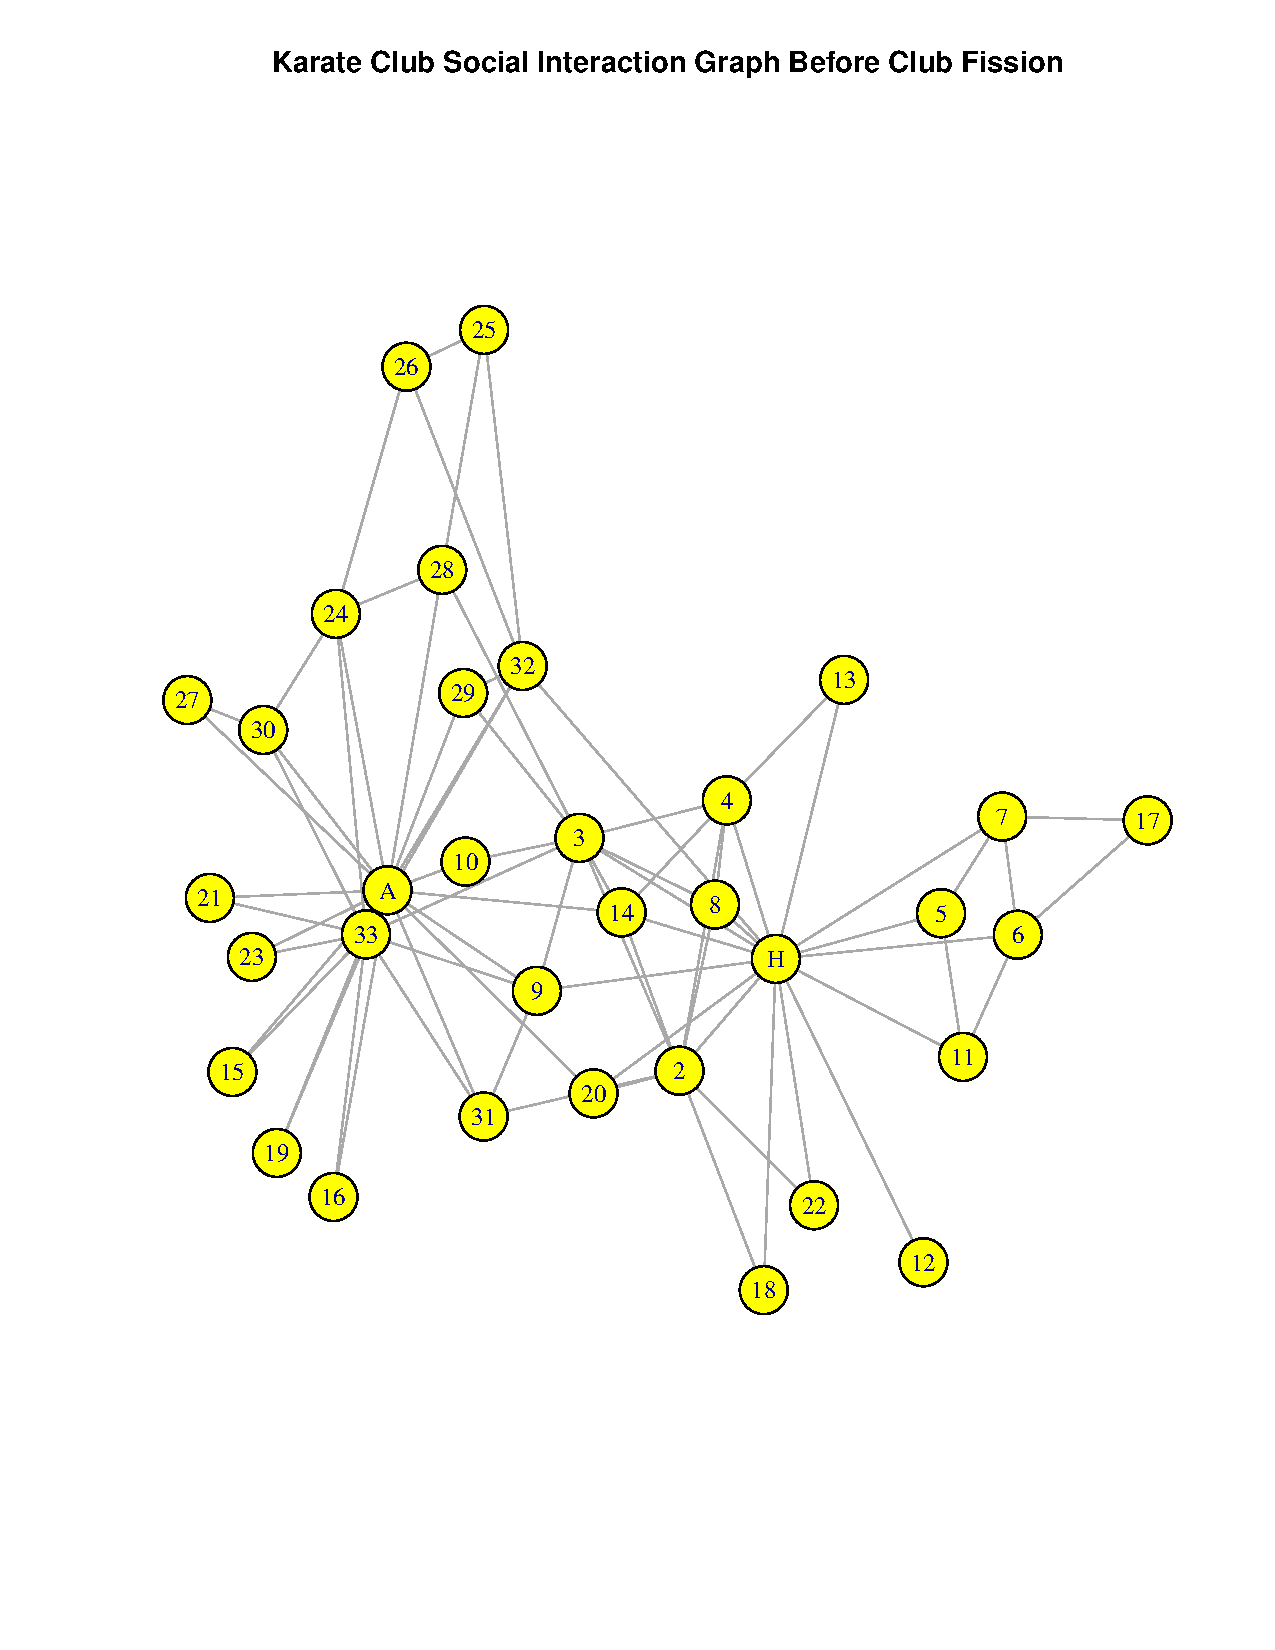
\includegraphics[scale=0.7]{before.pdf}
\end{figure}

\pagebreak

Now it's time to predict the result of the split of the Karate club using the edge-betweenness-community-detection algorithm and comparing the result to the actual split.

\begin{lstlisting}[language=R, breakatwhitespace=〈false), label=Predicted Karate Club Social Interaction Graph if the Club splits into 2 groups in R, caption= Predicted Karate Club Social Interaction Graph if the Club splits into 2 groups in R]
> library("igraph")
> library(igraphdata)
> data(karate)
> Karate_eb <- edge.betweenness.community(karate)
> groups <- cutat(Karate_eb, 2)
> colors <- cm.colors(2, 1)
> plot(karate, 
+      vertex.color=colors[groups],
+      vertex.size = 10,
+      main="Predicted Karate Club Social Interaction Graph if the Club splits into 2 groups"
+ )
>
\end{lstlisting}

\begin{figure}[H]
\centering
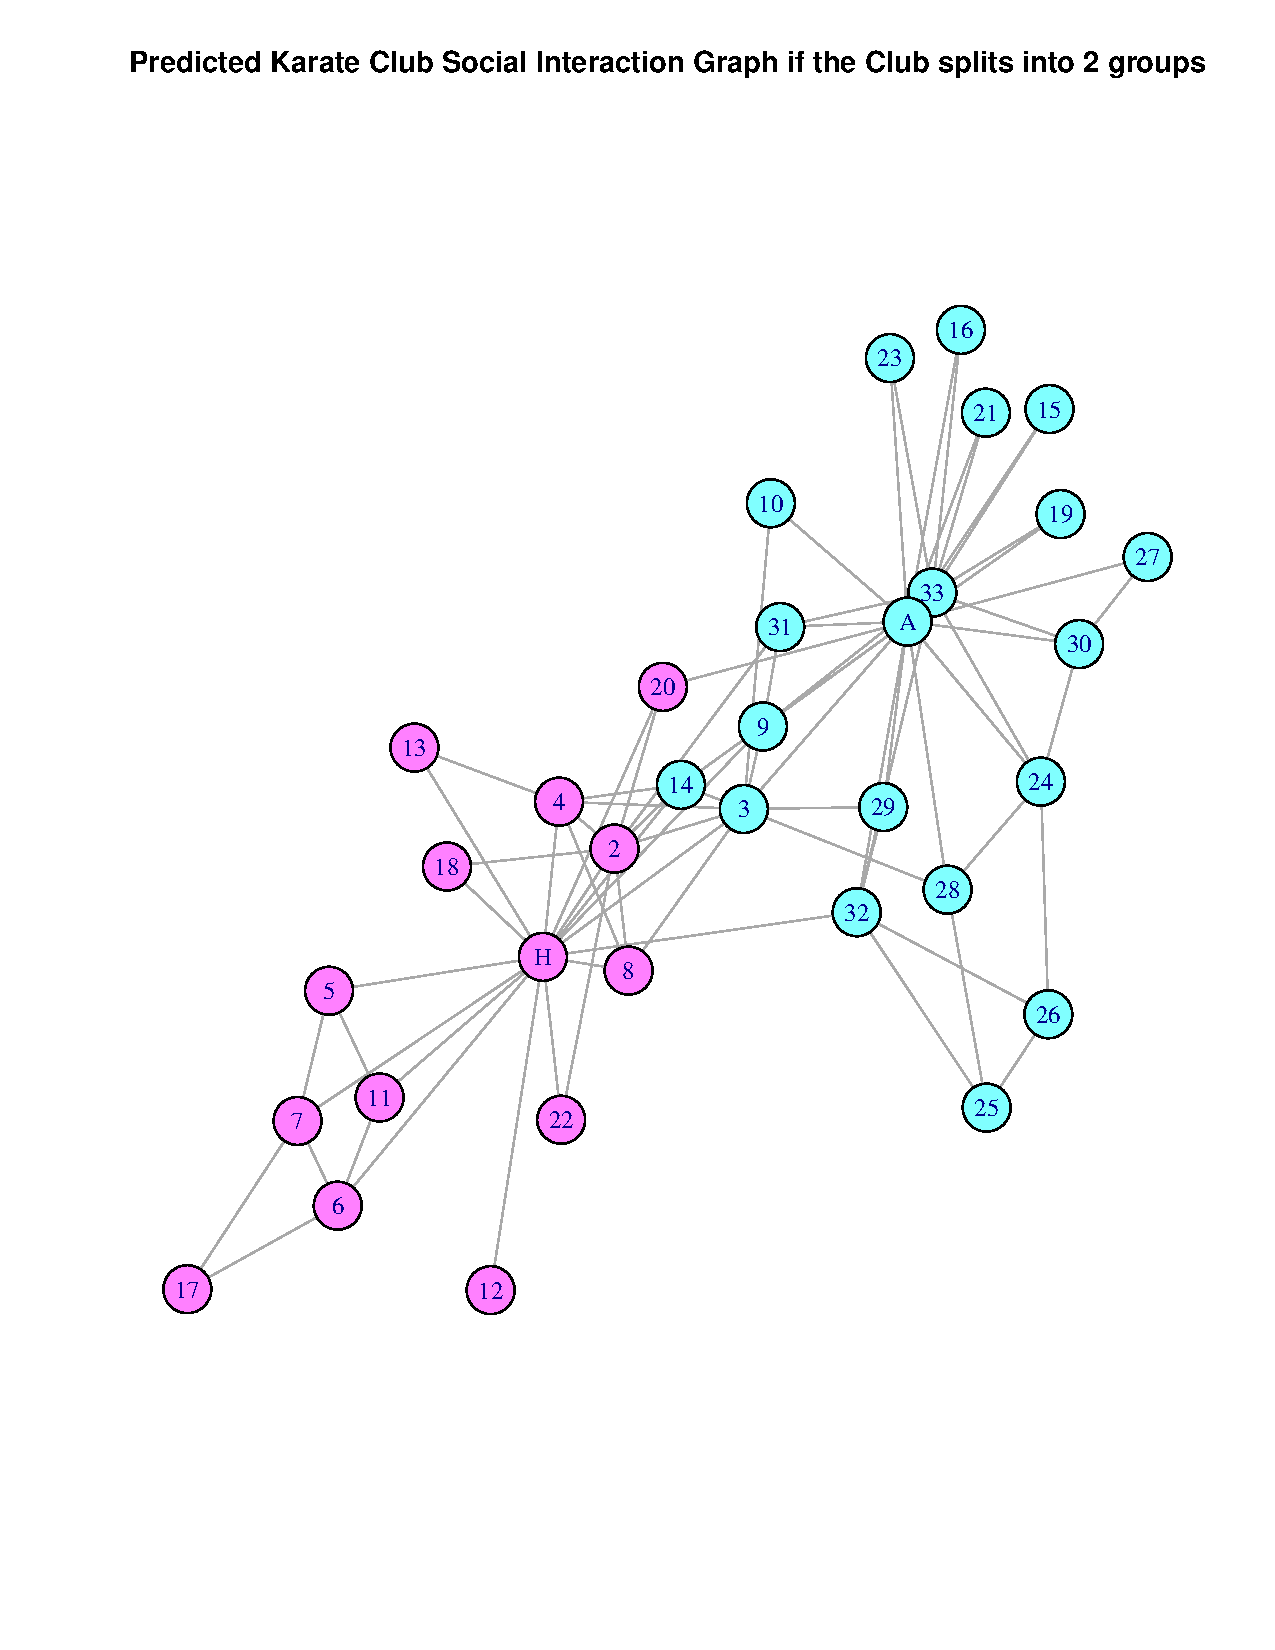
\includegraphics[scale=0.7]{2.pdf}
\end{figure}

\pagebreak

\textbf{The Actual Split:}
This image is taken from this link:

https://en.wikipedia.org/wiki/Zachary\%27s\_karate\_club

In this plot, node 1 stands for the instructor ``Mr. Hi'', node 34 for the president, ``John A''.

\begin{figure}[H]
\centering
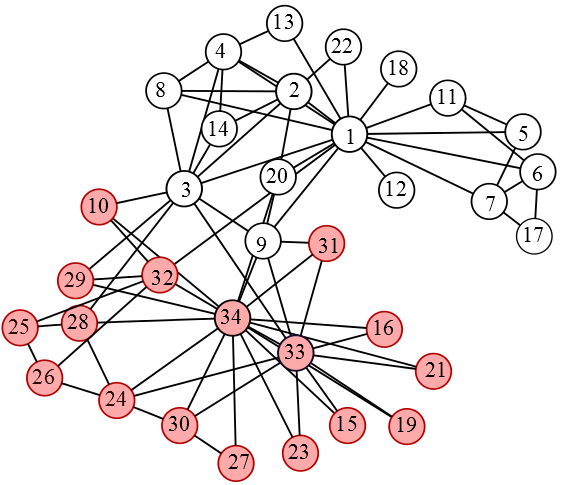
\includegraphics[scale=0.7]{after.png}
\end{figure}

Comparing the two previous graphs, we find that the number of misses is 3. The corresponding nodes are 3, 9, and 14.

\textbf{Computing the accuracy of our prediction:}

The error can be calculated by dividing the number of misses by the total number of nodes and multiply the result by 100.

$$ E = (M/T) \times 100 = 8.8\% $$

Therefore the accuracy of our prediction is 91.2\%

\subsection*{Included Files:}
Q1\_R\_Code.R, 2.pdf, after.png, before.pdf

\section*{Question 2:}
We know the group split in two different groups.  Suppose the
disagreements in the group were more nuanced -- what would the clubs
look like if they split into groups of 3, 4, and 5?

\subsection*{Answer:}
The prediction for the split of the karate club into more than two groups can be done in a similar fashion. Changing the R code accordingly gives us the desired graphs for the split into 3, 4, or 5 groups.

\begin{lstlisting}[language=R, breakatwhitespace=〈false), label=Predicted Karate Club Social Interaction Graph if the Club splits into 3 groups in R, caption= Predicted Karate Club Social Interaction Graph if the Club splits into 3 groups in R]
> library("igraph")
> library(igraphdata)
> data(karate)
> Karate_eb <- edge.betweenness.community(karate)
> groups <- cutat(Karate_eb, 3)
> colors <- terrain.colors(3, 1)
> plot(karate, 
+      vertex.color=colors[groups],
+      vertex.size = 10,
+      main="Predicted Karate Club Social Interaction Graph if the Club splits into 3 groups"
+ )
>
\end{lstlisting}

\begin{figure}[H]
\centering
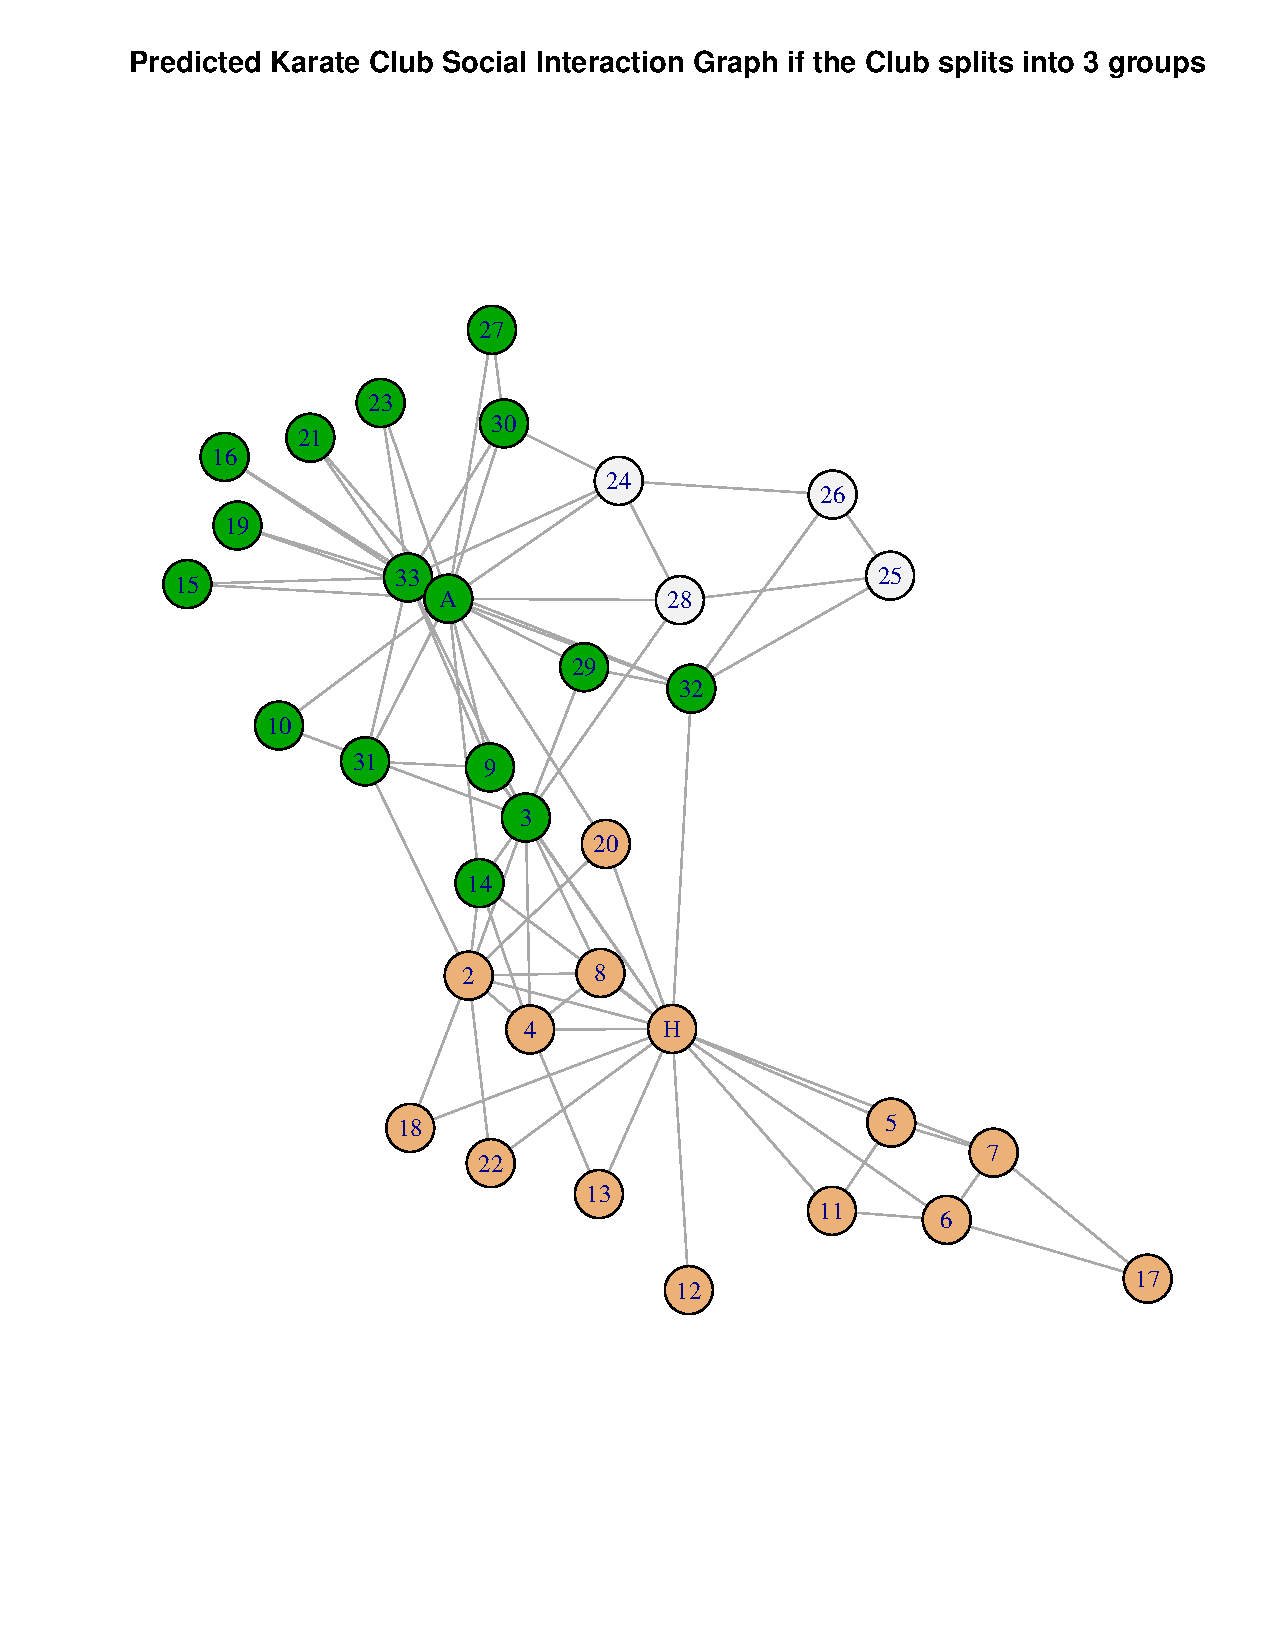
\includegraphics[scale=0.7]{3.pdf}
\end{figure}

\pagebreak

\begin{lstlisting}[language=R, breakatwhitespace=〈false), label=Predicted Karate Club Social Interaction Graph if the Club splits into 4 groups in R, caption= Predicted Karate Club Social Interaction Graph if the Club splits into 4 groups in R]
> library("igraph")
> library(igraphdata)
> data(karate)
> Karate_eb <- edge.betweenness.community(karate)
> groups <- cutat(Karate_eb, 4)
> colors <- terrain.colors(4, 1)
> plot(karate, 
+      vertex.color=colors[groups],
+      vertex.size = 10,
+      main="Predicted Karate Club Social Interaction Graph if the Club splits into 4 groups"
+ )
>
\end{lstlisting}

\begin{figure}[H]
\centering
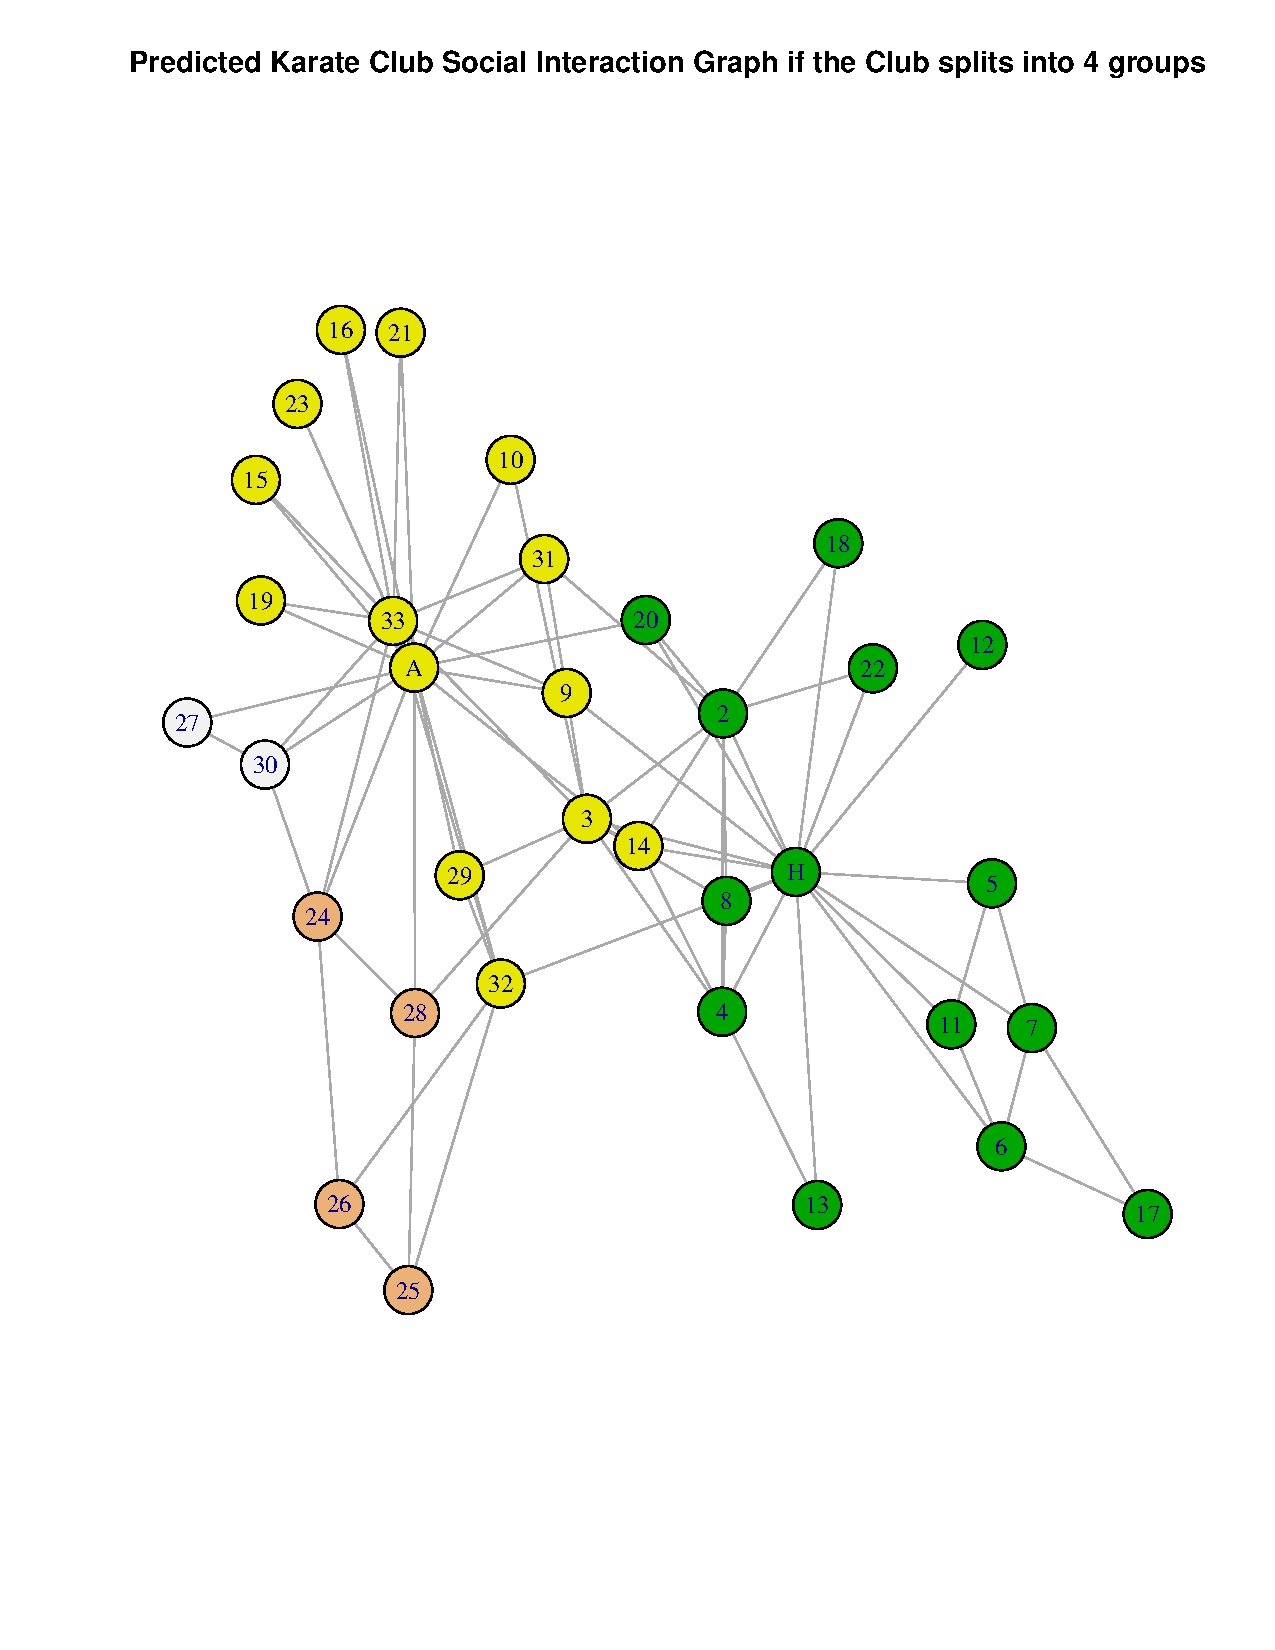
\includegraphics[scale=0.7]{4.pdf}
\end{figure}

\pagebreak


\begin{lstlisting}[language=R, breakatwhitespace=〈false), label=Predicted Karate Club Social Interaction Graph if the Club splits into 5 groups in R, caption= Predicted Karate Club Social Interaction Graph if the Club splits into 5 groups in R]
> library("igraph")
> library(igraphdata)
> data(karate)
> Karate_eb <- edge.betweenness.community(karate)
> groups <- cutat(Karate_eb, 5)
> colors <- terrain.colors(5, 1)
> plot(karate, 
+      vertex.color=colors[groups],
+      vertex.size = 10,
+      main="Predicted Karate Club Social Interaction Graph if the Club splits into 5 groups"
+ )
>
\end{lstlisting}

\begin{figure}[H]
\centering
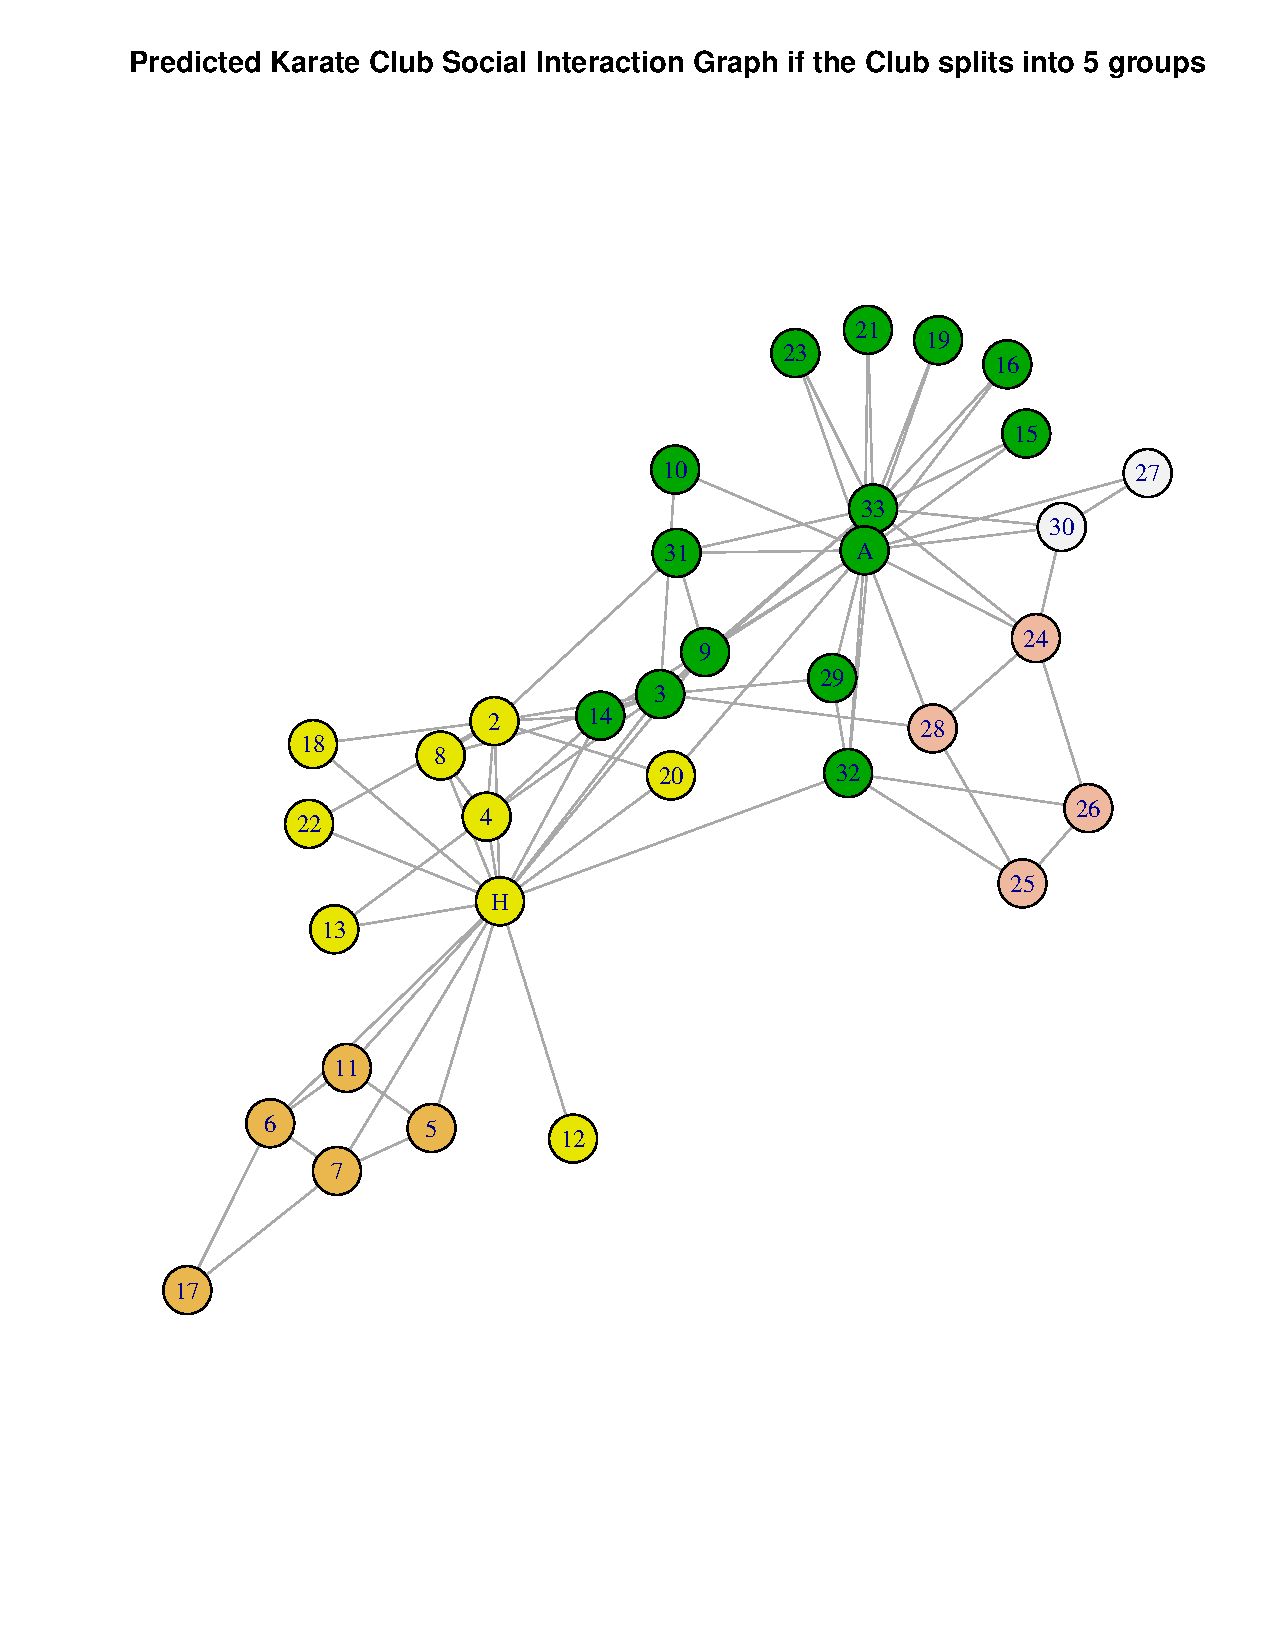
\includegraphics[scale=0.7]{5.pdf}
\end{figure}

\subsection*{Included Files:}
Q2\_R\_Code.R, 3.pdf, 4.pdf, 5.pdf

\end{document}
